\secnumbersection{MARCO CONCEPTUAL}

En el presente capítulo, se detallarán los conceptos fundamentales que son requeridos tanto para el desarrollo de la memoria, como también para el entendimiento de esta. Son definidos los conceptos como el framework \textit{robot operating system}, la robótica, los algoritmos de localización, mapeo y navegación y los ambientes de simulación gazebo y rviz.

\subsection{ROBÓTICA}
La concepción de la idea de una máquina que ayude al ser humano proviene del siglo 3 antes de Cristo, donde se concibe la primera idea de una máquina mecánica que esté creada con la única utilidad en ayudar al ser humano en sus actividades diarias. Sin embargo, la concepción moderna de robots proviene de la edad media con los autómatas de Da Vinci y Al Jazari, los cuales se consideran los primeros robots.
La robótica moderna es un área multidisciplinaria de la ingeniería en donde conjuntamente trabajan las ingenierías electrónica, mecánica, informática para el estudio, análisis, diseño y creación de máquinas autónomas capaces de realizar tareas asignadas o aprender mediante las realizan, tal y como lo muestra la Figura \ref{fig:areas_robotica}. 
\begin{figure}[h]
\centering
\includegraphics[width=0.5\textwidth]{figures/02marco_conceptual/robótica.png}
\caption{\label{fig:areas_robotica} Áreas de la Robótica} 
Fuente: \cite{area_rob_2017}
\end{figure}

\newpage
\subsection{ROBOT OPERATING SYSTEM}
\textit{Robot Operating System} (ROS) es un \textit{framework} orientado a la investigación en robótica. Si bien ROS no es un sistema operativo, provee de los servicios estándar de uno como el control de dispositivos de bajo nivel, la implementación de funcionalidad de uso común, abstracción de hardware, el envío de mensajes entre procesos, entre otros elementos. Está basado en una arquitectura de grafos en donde cada nodo implementa una funcionalidad específica, estos pueden recibir o enviar mensajes, controlar actuadores o sensores, comunicarse con otros nodos, entre otras funcionalidades.
ROS está compuesto por 3 conceptos esenciales que se nombraron anteriormente:
\begin{itemize}
    \item \textbf{Nodos: } Corresponden a los archivos ejecutables que utilizará ROS para realizar acciones. Los nodos se podrán comunicar con otros nodos mediante canales establecidos y el paso de mensajes estructurados.
    \item \textbf{Canales: } Corresponden a los diversos paradigmas de comunicación que se detallarán en la siguiente sección, mediante los cuales los nodos enviarán mensajes.
    \item \textbf{Mensajes: } Corresponden a datos estructurados mediante una cabecera y campos específicos, tales como enteros, flotantes, textos, entre otros.
\end{itemize}

\subsubsection{PARADIGMAS DE COMUNICACIÓN}
Para realizar la comunicación entre los nodos, ROS presenta 3 tipos de paradigmas de comunicación los cuales utilizan los protocolos TCP y UDP (TCPROS y UDPROS respectivamente) para realizar el intercambio de mensajes, tal como lo detalla Anis Koubaa en su libro \cite{anis_koubaa_robot_2016}.

\begin{itemize}
    \item \textbf{Topics: } El paradigma de comunicación \textit{Publisher - Subscriber} se presenta cuando uno de los nodos de ROS está publicando o está suscrito a un tópico el cual contiene un mensaje determinado, dicho mensaje está definido por un nombre y su contenido. Este, se envía por un tópico específico creando un canal de comunicación entre los nodos que lo necesiten. Esta comunicación se realiza solo en una dirección y se puede dar comunicación 1* a 1* \footnote{Soporta la comunicación 1 a 1, 1 a muchos y también muchos a 1}. Esta comunicación se puede ver descrita en la Figura \ref{fig:ROS_topics}.
    \begin{figure}[h]
    \centering
    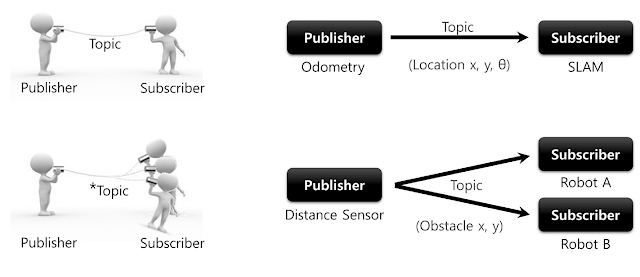
\includegraphics[width=0.7\textwidth]{figures/02marco_conceptual/ROS_topic.png}
    \caption{\label{fig:ROS_topics} Paradigma de comunicación - Topics} 
    Fuente: \cite{robin_robotics_2019}
    \end{figure}
    
    \item \textbf{Server Services: }
    El paradigma de comunicación \textit{Server Services} se plantea la utilización de un servidor donde el cliente envía una petición al servidor y el servidor le entrega una respuesta. Este paradigma de comunicación es síncrono, por lo que el cliente quedará esperando la respuesta del servidor y también es bidireccional a diferencia del anterior. Esta comunicación se puede ver descrita en la Figura \ref{fig:ROS_services}.
    
    \begin{figure}[h]
    \centering
    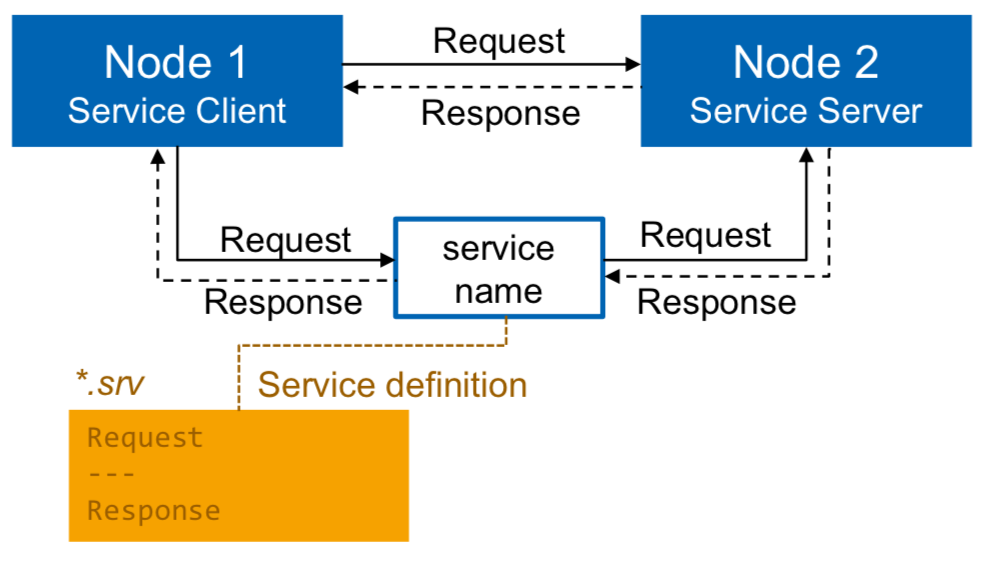
\includegraphics[width=0.7\textwidth]{figures/02marco_conceptual/ROS_service.png}
    \caption{\label{fig:ROS_services} Paradigma de comunicación - Server Services} 
    Fuente: \cite{ros_services_2018}
    \end{figure}
    
    \item \textbf{Server Actions: }
    El paradigma de comunicación \textit{Server Actions} al igual que el paradigma descrito anteriormente, plantea la utilización de un servidor donde el cliente envía una petición al servidor y el servidor le entrega una respuesta, sin embargo, esta vez la comunicación es asíncrona, por lo que el cliente puede seguir realizando sus tareas sin esperar la respuesta del servidor. Esta comunicación se puede ver descrita en la Figura \ref{fig:ROS_actions}.
    
    \begin{figure}[h]
    \centering
    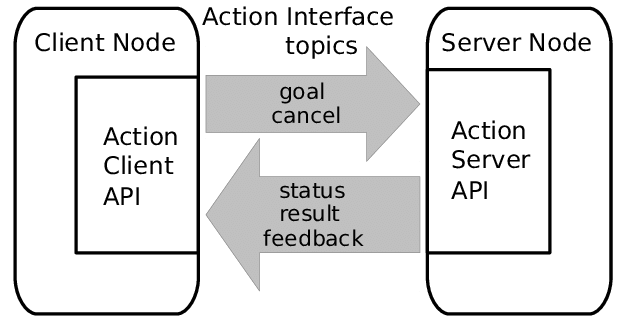
\includegraphics[width=0.7\textwidth]{figures/02marco_conceptual/ROS_action.png}
    \caption{\label{fig:ROS_actions} Paradigma de comunicación: Server Actions} 
    Fuente: \cite{andres_rosoclingo_2013} 
    \end{figure}
    \end{itemize}
    
    Cada uno de estos paradigmas de comunicación se utilizarán en el robot para enviar mensajes entre los actuadores y el procesador principal, para enviar la imagen que se está observando al computador, para controlar el robot, enviar coordenadas, observar el mapa que se está creando, la ruta definida, entre otras tareas y análisis que se realizarán.

\newpage
\subsection{SIMULACIÓN}
La simulación es un elemento no menor en el área de la robótica, ya que permite testear de manera segura los robots diseñados, permite utilizar los algoritmos creados, analizar el comportamiento del robot sin comprometer su estructura física y verificar los posibles errores que se pueda observar. Dentro del estado del arte de la robótica móvil, los dos motores gráficos que se utilizan por excelencia son \textit{Gazebo} y \textit{RVIZ}. Takaya presenta una aproximación sobre como simular entornos y probar robots utilizando Gazebo \cite{takaya_simulation_2016} y las bases necesarias para testear algoritmos de localización y navegación en entornos controlados.

\subsubsection{GAZEBO}
Gazebo es un  software de \textit{open source} diseñado para simplificar el desarrollo de robots y aplicaciones de alto rendimiento. Está basado en la arquitectura \textit{cliente/servidor}. Se presenta esta arquitectura como la comunicación de dos actores, el cliente el cual consume los recursos y el servidor el cual provee dichos recursos \cite{lizama_redes_nodate}. Gazebo es considerado el simular más importante en la industria de la robótica, donde se pueden simular entornos complejos, físicas realísticas para una mayor semejanza con las aplicaciones reales del robot y estructuras complejas como se muestra en la Figura \ref{fig:ROS_gazebo}. Es esencialmente usado en el área de la investigación cuando no se dispone físicamente del robot y se requiere testear los algoritmos creados o el comportamiento del robot, por lo que se simula el entorno real y lo que el robot está efectivamente viendo.


\begin{figure}[h]
    \centering
    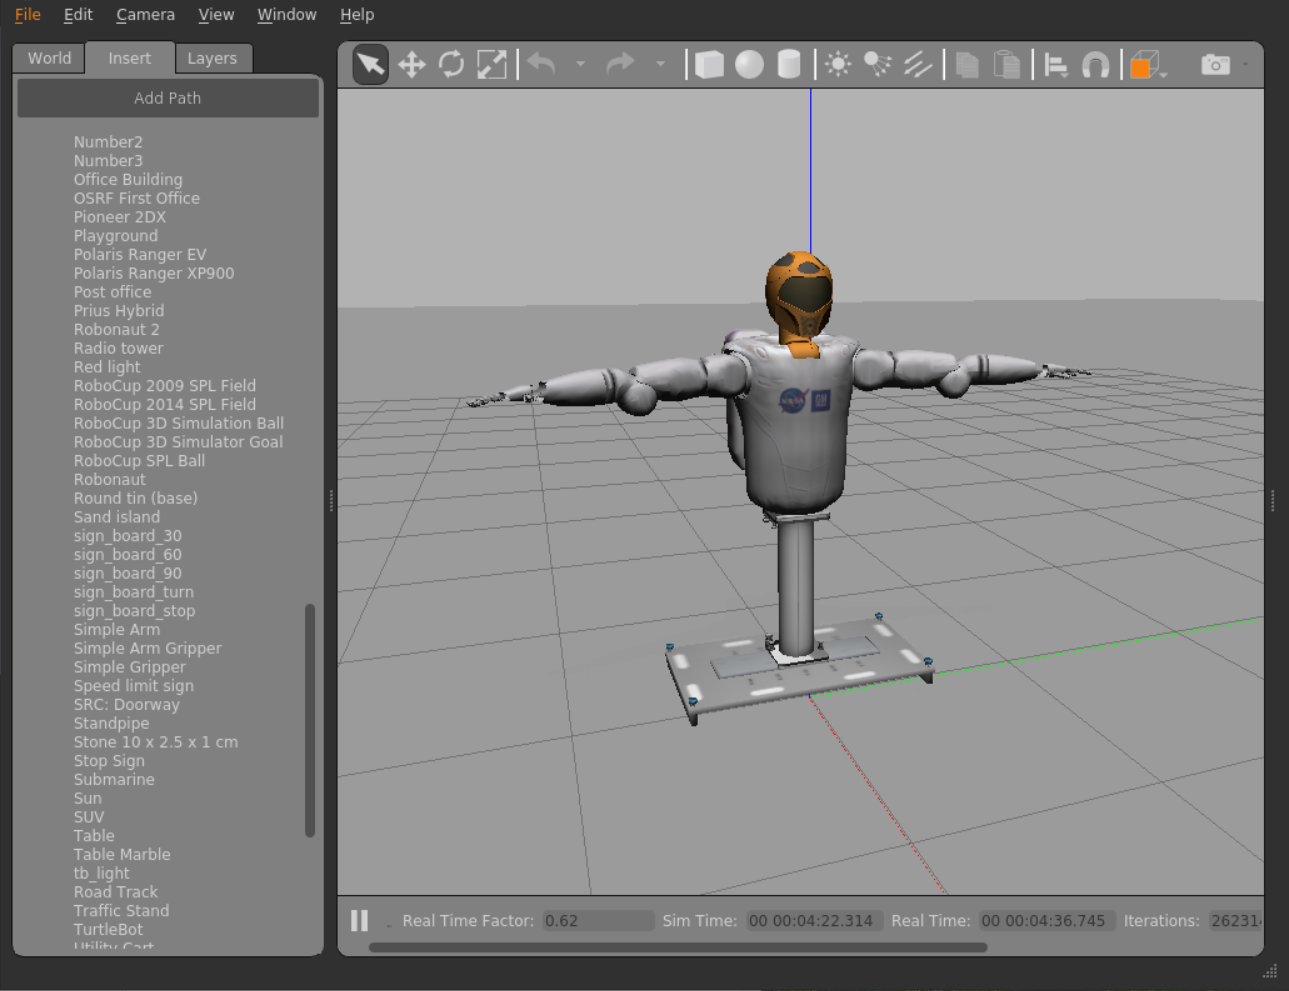
\includegraphics[width=0.5\textwidth]{figures/02marco_conceptual/Gazebo.PNG}
    \caption{\label{fig:ROS_gazebo} Robonauta 2 de la NASA simulado en Gazebo} 
    Fuente: \textit{Fabricación propia}
    \end{figure}

\subsubsection{RVIZ}
\textit{Robot Visualizer} o Rviz es una interfaz gráfica tridimensional de ROS que permite observar datos, mensajes, estados en tiempo real y otros elementos, de lo que cree el robot que está ocurriendo. El simulador permite la integración con la información recibida por los diversos paradigmas de ROS descritos anteriormente, como también es posible su integración con la información provista por Gazebo, lo que permite testear los algoritmos utilizando tanto Gazebo si no se tiene acceso al robot físico o también utilizando el robot real \cite{kam_rviz_2015}. Se puede observar en la Figura \ref{fig:ROS_rviz} en la sección central como Rviz presenta el mapa generado por el robot y en su extremo izquierda, la información provista por Gazebo mediante una cámara dispuesta en el robot.

\begin{figure}[h]
    \centering
    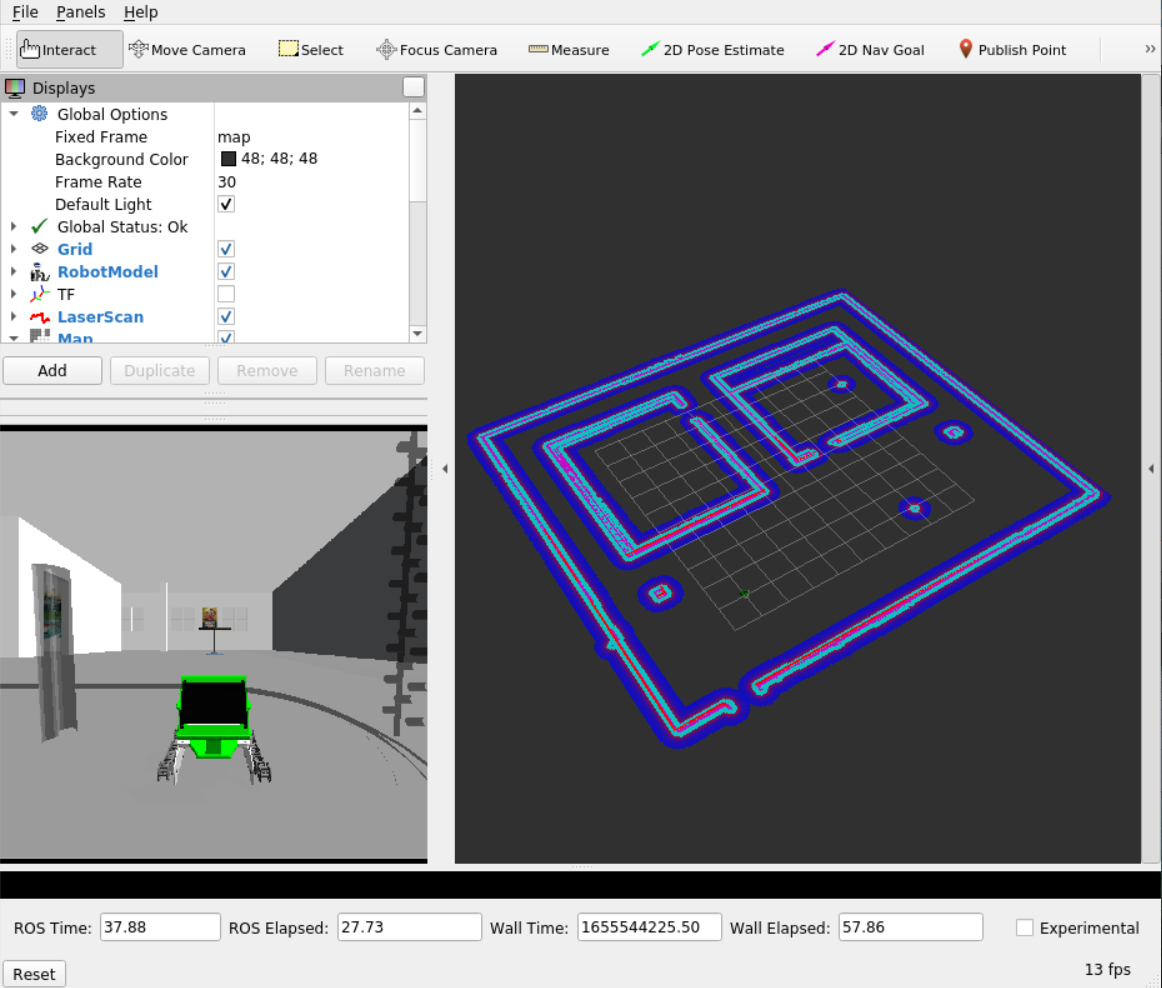
\includegraphics[width=0.5\textwidth]{figures/02marco_conceptual/Rviz.PNG}
    \caption{\label{fig:ROS_rviz} Visualización del entorno gráfico Rviz} 
    Fuente: \textit{Fabricación propia}
    \end{figure}
    
\newpage
\subsection{ALGORITMOS DE LOCALIZACIÓN}
La localización en el área de la robótica es la tarea de determinar en donde se encuentra el robot con respecto a su entorno. En el área de la robótica móvil es una de las tareas fundamentales a la hora de realizar un robot autónomo. En un escenario típico de localización se dispone del mapa del entorno y a través de la información recopilada por los sensores, el robot debe estimar su posición y orientación dentro del entorno \cite{huang_robot_2016}. Dentro de los algoritmos clásicos de localización utilizados en el estudio de la robótica móvil son los algoritmos \textit{Markov, Grid y Monte Carlo} los cuales se detallan en las siguientes secciones.


\textbf{ALGORITMO MARKOV}

El algoritmo Markov fue propuesto por primera vez en el año 1960 para el reconocimiento del habla, sin embargo, con el pasar de los años las aplicaciones del algoritmo se han expandido a diversas áreas, siendo una de esas la robótica \cite{reyes_mobile_2015}. Dicho algoritmo se basa en la información provista por los sensores y genera un modelo probabilístico de la localización del robot en su entorno y de esta manera el algoritmo entrega las posibles posiciones en donde el robot se puede encontrar. En el Algoritmo  \ref{alg:Algoritmo_Markov} se puede apreciar en detalle el funcionamiento del algoritmo.

\begin{algorithm}[H]
\centering
    \begin{algorithmic}[1]
        \Require $bel(x_{t1}), u_{t}, z_{t}, map$ 
        \vspace{1mm}
        \hline
        \vspace{1mm}
           \ForAll{$x_t$}
            $\overline{bel} = $∫p(x_{t}|u_{t},x_{t-1},m) \cdot bel(x_{t-1}) \partial(x_{t-1})$
            \State $bel(x_{t}) = \eta \cdot p(z_{t}|x_{t}, m) \cdot $\overline{bel(x_{t})}$
           \EndFor
           
        \State \Return $bel(x_{t})$
        \vspace{1mm}
        \hline
        \vspace{1mm}
    \end{algorithmic}
\caption{Pseudocódigo algoritmo Markov}
Fuente: \cite{thrun_probabilistic_2005}
\label{alg:Algoritmo_Markov}
\end{algorithm}

Este se deriva a partir del algoritmo Bayesiano, es decir, se requiere una posición inicial ($Bel(x_{t1}$), la cual mientras más certera mejor será el desempeño del algoritmo, con la diferencia de que el algoritmo de Markov también requiere el mapa ($map$) del entorno. Luego por cada posición el algoritmo iterará para entregar el modelo probabilístico con respecto a la localización del robot. Autores como Rajesh Kannan han utilizado el algoritmo para realizar un control mediante comandos de voz \cite{megalingam_ros_2019} siguiendo la estructura anteriormente dicha.

\textbf{ALGORITMO GRID}

El algoritmo aproxima la posición utilizando un filtro de histograma sobre una descomposición en la posición espacial. La versión más básica mostrada en el Algoritmo \ref{alg:Algoritmo_Grid} consta de una división del entorno mediante grillas del mismo tamaño y de la probabilidad de que el robot se encuentre en dicha grilla mediante la información provista por los sensores, es esencial entregar al algoritmo el tamaño de las cuadrículas ya que un tamaño menor indica mayor precisión a cambio de un mayor tiempo de localización. También el algoritmo toma en cuenta el modelo del movimiento del robot \textit{motion\_model} y la información provista por los sensores mediante \textit{measurement\_model}. Una aproximación del algoritmo es implementado por Zengfeng Wang en \cite{wang_grid-based_2018}, en donde mediante la información provista por sensores inalámbricos se logra localizar en el entorno.

\begin{algorithm}[H]
\centering
    \begin{algorithmic}[1]
        \Require $\{p_{k,t-1}\}, u_{t}, z_{t}, m$ 
        \vspace{1mm}
        \hline
        \vspace{1mm}
           \ForAll{$k$}
           $\overline{p}_{k,t} = $ \sum_{i=0}^{n} p_{i,t-1} \textbf{motion\_model}(mean($x_{k}$), $u_{t}$,mean($x_{i}$)) 
            \State $p_{k,t} = \eta \cdot \overline{p}_{k,t}$ \textbf{measurement\_model}($z_{t}$, mean($x_{k}$), m))
            
           \EndFor
        \Return $\{p_{k,t}\}$
        \vspace{1mm}
        \hline
        \vspace{1mm}
    \end{algorithmic}
\caption{Pseudocódigo algoritmo Grid}
Fuente: \cite{thrun_probabilistic_2005}
\label{alg:Algoritmo_Grid}
\end{algorithm}


\textbf{ALGORITMO MONTE CARLO}

El MCL (Algoritmo Monte Carlo de Localización) es uno de los más populares e importantes entre los algoritmos de localización. Funciona a través de una probabilidad mediante partículas y se puede utilizar para la localización global y local \footnote{La localización global se utiliza al inicio, para encontrar la posición inicial del robot y la localización local se utiliza una vez que el robot empieza a moverse y se desea saber su posición durante el experimento.}. El modelo básico del MCL es un método no determinista utilizado para aproximar expresiones matemáticas complejas. Este método aplicado a la localización del robot se puede observar en el Algoritmo \ref{alg:Algoritmo_Monte_Carlo} en donde se encuentra la probabilidad de que el robot se encuentre en una posición mediante la información provista por sensores. El algoritmo se inicia con una serie de candidatos posibles de posición inicial y mediante nueva información provista por los sensores, el algoritmo determina la probabilidad de que el robot se encuentre en una determinada posición (las probabilidades bajas son eliminadas de la lista de posibles posiciones). Xiaoyu Wang muestra una posible implementación del algoritmo MCL modificado para la localización de un robot en un entorno controlado, realizando pruebas para la localización fija, mediante movimiento y el análisis de la localización una vez que el robot se mueve externamente de su posición
\cite{xiaoyu_adaptive_2018}.


\begin{algorithm}[H]
\centering
    \begin{algorithmic}[1]
        \Require $X_{t-1}, u_{t}, z_{t}, m$
        \vspace{1mm}
        \hline
        \vspace{1mm}
        \State $\overline{X}_{t} = X_{t} = \emptyset$
           \For{$m=1$ to $M$}
           \State $x_{t}^{[m]} =  $\textbf{ sample\_motion\_model}($u_{t}, x_{t-1}^{[m]} $)
           \State $w_{t}^{[m]} = $\textbf{ measurement\_model}($z_{t}, x_{t}^{[m]}, m $)
           \State $\overline{X}_{t} = \overline{X}_{t} + <x_{t}^{[m]}, w_{t}^{[m]}>$
           \EndFor
           \For{$m=1 $ to $M$}
           \State draw $i$ with probability \infty  $ w_{t}^{[i]}$
           \State add $w_{t}^{[i]}$ to $X_{t}$
           \EndFor
        \State \Return $X_{t}$
        \vspace{1mm}
        \hline
        \vspace{1mm}
    \end{algorithmic}
\caption{Pseudocódigo algoritmo Monte Carlo}
Fuente: \cite{thrun_probabilistic_2005}
\label{alg:Algoritmo_Monte_Carlo}
\end{algorithm}

\newpage
\subsection{ALGORITMOS DE MAPEO}
En la sección anterior se nombró que una de las tareas esenciales en la robótica móvil es la de localizarse en un entorno, ya que esto es clave para permitir la autonomía y lograr realizar las tareas asignadas, sin embargo, los algoritmos anteriormente descritos presentan un elemento en común, que es el parámetro del mapa. Un mapa construido adecuadamente es esencial para una correcta localización. La construcción del mapa supone crear una imagen 2D del entorno, de esta manera se visualizarán correctamente los objetos fijos como las murallas, objetos, estantes, entre otros. Existe una variación de un mapeo 3D planteado por Manuel González \cite{dos_reis_quantitative_2019}, en donde se observan las cualidades de generar un mapa tridimensional del entorno en donde se ubique el robot. El algoritmo más importante es el \textit{Grid Mapping} el cual es descrito en la siguiente sección y que dio pasos a otros algoritmos de mapeos como lo es el algoritmo \textit{Hector Mapping}, descrito a continuación. \footnote{Si bien existen otros importantes como GraphSLAM y FastSLAM, estos se detallarán en la sección de algoritmos SLAM debido a la utilización de dicha técnica.}

\textbf{ALGORITMO GRID MAPPING}

El algoritmo Grid Mapping es el algoritmo estrella entre los algoritmos de mapeos debido a la simpleza de su funcionamiento. Se basa en la probabilidad de que una celda esté ocupada o no según los datos que se reciben por parte de los sensores. El algoritmo básico se puede observar en el Algoritmo \ref{alg:Algoritmo Grid Mapping} en donde esencialmente se utiliza la información provista por los sensores para generar el mapa correspondiente. En caso que el sensor detecte un objeto, la casilla se marcara y en caso contrario se mantendrá desocupada \cite{sankalprajan_comparative_2020}. 

\begin{algorithm}[H]
\centering
    \begin{algorithmic}[1]
        \Require $\{l_{t-1},i\}, x_{t}, z_{t}$
        \vspace{1mm}
        \hline
        \vspace{1mm}
        \ForAll{cells $m_{i}$}
            \If{$m_{i}$ in perceptual field of $z_{i}$}
                \State $l_{t,i} = l_{t-1,i} $ + \textbf{inverse\_sensor\_model}($m_{i}, x_{t}, z_{t}$)
            \Else{$l_{t,i} = l_{t-1, i}$}
            \EndIf
        \EndFor
        \State \Return $\{l_{t,i}\}$
        \vspace{1mm}
        \hline
        \vspace{1mm}
    \end{algorithmic}
\caption{Pseudocódigo algoritmo GMapping}
Fuente: \cite{thrun_probabilistic_2005}
\label{alg:Algoritmo Grid Mapping}
\end{algorithm}

Un ejemplo visual del algoritmo se puede observar en la Figura \ref{fig:GMapping} en donde se observa a la izquierda el mapa real del entorno y a la derecha el mapa generado por el algoritmo.

\begin{figure}[H]
    \centering
    \begin{subfigure}[b]{0.40\textwidth}
    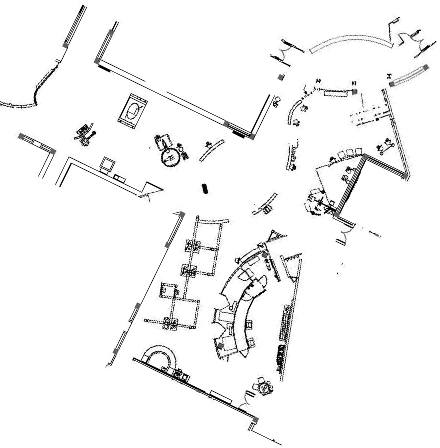
\includegraphics[width=\textwidth, height=\textwidth]{figures/02marco_conceptual/Mapa.PNG}
    \caption{Mapa del entorno}
    \label{fig:gmapping_sim}
    \end{subfigure}
    \begin{subfigure}[b]{0.40\textwidth}
    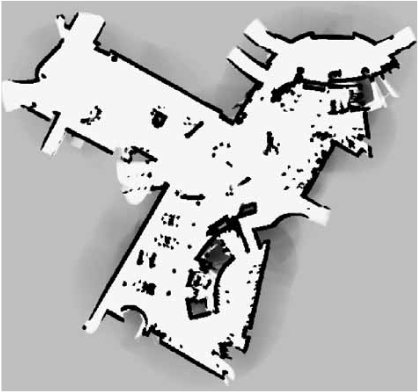
\includegraphics[width=\textwidth, height=\textwidth]{figures/02marco_conceptual/Mapa_generado.PNG}
    \caption{Mapa generado por GMapping}
    \label{fig:gmapping_map}
    \end{subfigure}
    \caption{Comparación entre el mapa real del entorno y el mapa generado por el algoritmo GMapping}
    Fuente: \cite{thrun_probabilistic_2005}
    \label{fig:GMapping}
\end{figure}

\textbf{ALGORITMO HECTOR MAPPING}

El algoritmo Hector Mapping, propuesto por Stefan Kohlbrecher y Oskar von Stryk en \cite{kohlbrecher_flexible_2011}, en donde se propone un algoritmo lo suficientemente preciso que tenga bajos requisitos tanto económicos, como computacionales. Al utilizar pocos recursos computacionales, dicho algoritmo es escalable a cualquier computador con procesadores de bajo peso y sobretodo, bajo consumo. Los resultados del mapeo utilizando el algoritmo sobre un ambiente simulado se pueden observar en la Figura \ref{fig:hector_slam_work}.

\begin{figure}[H]
    \centering
    \begin{subfigure}[b]{0.40\textwidth}
    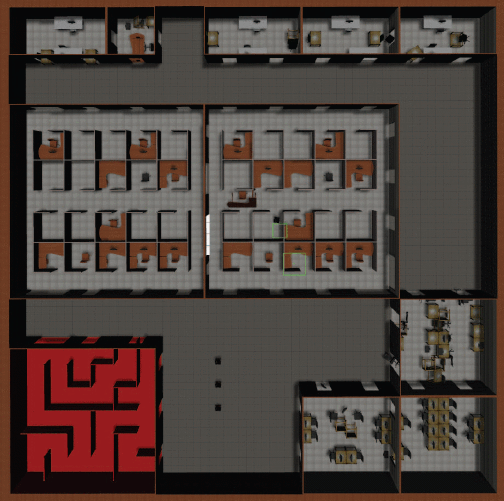
\includegraphics[width=\textwidth, height=\textwidth]{figures/02marco_conceptual/hector_slam_simulation.png}
    \caption{Ambiente simulado}
    \label{fig:hector_slam_sim}
    \end{subfigure}
    \begin{subfigure}[b]{0.40\textwidth}
    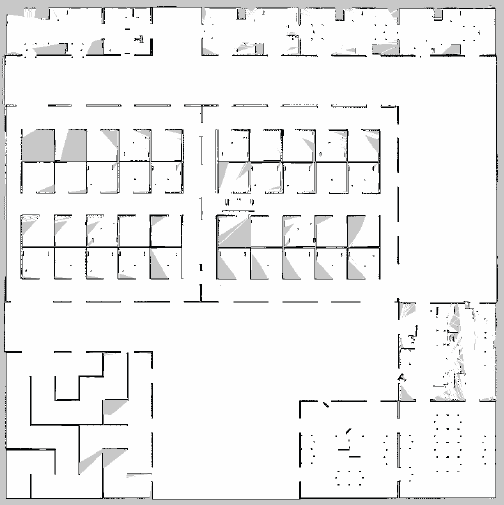
\includegraphics[width=\textwidth, height=\textwidth]{figures/02marco_conceptual/hector_slam_map.png}
    \caption{Mapa generado por Hector Mapping}
    \label{fig:hector_slam_map}
    \end{subfigure}
    \caption{Comparación entre el ambiente simulado y el mapa generado por el algoritmo Hector Mapping}
    Fuente: \cite{kohlbrecher_flexible_2011}
    \label{fig:hector_slam_work}
\end{figure}

Si bien existen variaciones del algoritmo Hector Mapping, ya que el gran beneficio del algoritmo es su capacidad de adaptarse a las distintas necesidades del sistema, el funcionamiento básico es el mismo en todos los casos y se puede observar en el Algoritmo \ref{alg:Algoritmo Hector Mapping}, en donde, al solo utilizar información del lidar se realiza la corrección del mapa. 

\begin{algorithm}[H]
\centering
    \begin{algorithmic}[1]
        \Require $HT_j, RT_J, Iter$
        
        \Ensure $TMatrix$
        \vspace{1mm}
        \hline
        \vspace{1mm}
        \State $MinResidual \leftarrow 1$

        \Function {MATCHFINDER}{$TransMx, HT_j, RT_j$}
            \While{$i<Iter$}
                \State $TMatrix \leftarrow$ ORIENICP($HT_j, RT_j$)
            \EndWhile
        \EndFunction
        
        \Function {ORIENICP}{$HT_j, RT_j$}
            \State $i \leftarrow 0$
            \State $HPoints \leftarrow HT_j$
            \State $RPoints \leftarrow RT_j$
            \State $MinResidual \leftarrow ICP(Hpoints, RPoints)$
            \If {$ORIENICP.Residual < MinResidual$} 
                \State $Trans \leftarrow ICP(Hpoints, RPoints)$
                \State $MinResidual \leftarrow OrienICP.Residual$
                \State \Return{$Trans$}
            \Else
                \State $PASS$
           \EndIf
        \EndFunction
        
        \Function {ALIGNORIENT}{$TransMX, Pose$}
            \State \hspace{4mm} $Pose[x,y].Rotate(TransMx)$
            \State \hspace{4mm} $Pose[x,y].Translate(TransMx)$
            
        \EndFunction
        \vspace{1mm}
        \hline
        \vspace{1mm}
    \end{algorithmic}
\caption{Pseudocódigo algoritmo Hector Mapping}
Fuente: \cite{kohlbrecher_flexible_2011}
\label{alg:Algoritmo Hector Mapping}
\end{algorithm}

\newpage
\subsection{ALGORITMOS DE NAVEGACIÓN}

Una vez que se ha construido el mapa y el robot se puede localizar en este, es necesario contar con algoritmos de navegación que permitan integrar la información provista por los algoritmos anteriormente señalados y así navegar por el entorno, es decir, a partir de la posición inicial y una posición final u objetivo, debe planificar la mejor ruta (esto puede ser en términos de eficiencia, costes, riesgos, entre otros) y realizar la ruta pertinente \cite{gul_comprehensive_2019}. El funcionamiento básico de un algoritmo de navegación debe en primera instancia dividir el mapa generado por los algoritmos de mapeo en cuadrículas \footnote{La división del mapa se puede realizar de manera discreta o de manera probabilística según se determine dentro del algoritmo} y determinar la ruta óptima como se observa en la Figura \ref{fig:ROS_navegacion}.

\begin{figure}[h]
    \centering
    \includegraphics[width=0.8\textwidth]{figures/02marco_conceptual/Navegación.PNG}
    \caption{\label{fig:ROS_navegacion} Cuadrícula de navegación} 
    Fuente: \cite{thrun_probabilistic_2005}
\end{figure}

Uno de los algoritmos clásicos de navegación y planeamiento de rutas es el A*, la versión básica del algoritmo que se puede observar en el Algoritmo \ref{alg:Algoritmo A*}. Consta de una cuadrícula o mapa, una posición inicial y una posición final, está diseñado de tal manera que si bien la solución encontrada no es la mejor, si es encontrada de manera rápida, por lo que se considera que la solución encontrada es un máximo óptimo. Existen variaciones como las identificadas en \cite{noauthor_global_nodate}, sin embargo, parte del algoritmo básico de la búsqueda A*.

\begin{algorithm}[H]
\centering
    \begin{algorithmic}[1]
        \Require $start, goal$
        \vspace{1mm}
        \hline
        \vspace{1mm}
        \State open\_list =  containing start
        \State  closed\_list = $\emptyset$
        \State  start.g = 0
        \State start.f = start.g + heuristic(start,goal)
        \While{ current is not goal}
            \State current = open\_list element with lowest f cost
            \State remove current from open\_list
            \State add current to closed\_list
            \ForAll{neighbor of current}
                \If{neighbor not in closed\_list}
                    \State neighbor.f = current.g + heuristic(neighbor, goal)
                    \If{neighbor is not in open\_list}
                        \State add neighbor to open\_list
                    \Else
                        \State openneighbor = neighbor in open\_list
                        \If{neighbor.g < openneighbor.g}
                            \State openneighbor.g = neighbor.g
                            \State openneighbor.parent = neighbor.parent
                        \EndIf
                    \EndIf
                \EndIf
                \If{$open\_list$ $is$ $\emptyset$}
                    \State \Return $false$
                \EndIf
                \State \Return{backtrack\_path(goal)}
            \EndFor
        \EndWhile
        \vspace{1mm}
    \hline
    \vspace{1mm}
    \end{algorithmic}
\caption{Pseudocódigo algoritmo A*}
Fuente: \cite{candra_application_2021}
\label{alg:Algoritmo A*}
\end{algorithm}

\newpage
\subsection{ESTADO DEL ARTE}

Las aplicaciones de la robótica móvil se dan en múltiples áreas, por ejemplo, en la exploración minera ayudando a extraer datos de la superficie, también se pueden dar en la exploración planetaria con los \textit{rovers} enviados a Marte. Operando en misiones de rescate y búsqueda de personas, reconocimiento de terreno, investigación militar, entre otros rubros más \cite{russell_artificial_2010}.

Es así como los robots móviles se definen como un \textit{``Un sistema electromecánico capaz de desplazarse de manera autónoma sin estar sujeto físicamente a un solo punto. Posee sensores que permiten monitorear a cada momento su posición relativa a su punto de origen y a su punto de destino. Normalmente su control es en lazo cerrado. Su desplazamiento es proporcionado mediante dispositivos de locomoción, tales como ruedas, patas, orugas, etc.''} \cite{sotelo_robots_2007}. 

En grandes rasgos los robots móvil se pueden identificar según el mecanismo que se utilice para realizar el movimiento, entre los cuales se destacan 3 grupos: Mediante ruedas, mediante extremidades y mediante orugas. Shigeo Hirose \cite{hirose_three_1991} describe como una primera aproximación la existencia de dichos grupos y los identifica de la siguiente manera:
\begin{itemize}
    \item \textbf{Aquellos robots que utilizan ruedas o una combinación de estas para desplazarse.} Si bien su implementación es más sencilla, están limitados por su adaptabilidad al terreno, sin embargo, son bastante eficientes en los terrenos parejos o con pequeñas elevaciones.
    \item \textbf{Aquellos robots que presentan piernas o extremidades para trasladarse.} Los robots que basan su movilidad en piernas, pueden adaptarse al entorno y este pasa a un segundo plano cuando se tienen altos grados de libertad, sin embargo, no son eficientes en términos energéticos, pero si les permiten mayor movilidad.
    \item \textbf{Aquellos robots que presentan articulaciones que les permiten reptar como las serpientes u otros reptiles para realizar el movimiento.} Este tipo de robots están compuestos por una serie de articulaciones independientes lo que les permite mayor facilidad de transporte. Usualmente tienen un cuerpo radial pequeño y largo, y el tamaño les permite adentrarse en entornos en que otros robots no pueden hacerlo.
\end{itemize}

Años más tarde, Farbod Fahimi \cite{fahimi_autonomous_2009} cataloga al primer grupo, es decir, a los robots que utilizan ruedas, en 2 nuevos grupos: los robots móviles \textit{hillary-type} y los \textit{car-like}. Por una parte los primeros se caracterizan por tener dos o más ruedas motrices independientes, mientras que por otra parte los segundos se caracterizan por tener un solo motor que alimenta a las ruedas y por ende el movimiento viene dado por un solo elemento.

Actualmente podemos encontrar robots en los hogares que facilitan la vida, como las aspiradoras roomba, robots que despachan pedidos en almacenes o incluso robots que en restaurantes van a dejar comida a la mesa, por lo que se estima que un porcentaje no menor de la población mundial tendrá contacto con robots dentro de la siguiente década. En esta línea se observa que los potenciales beneficiarios de un robot móvil es un grupo no menor de personas como lo pueden ser los dueños de casas, familias con adultos mayores, doctores y enfermeras en hospitales, restaurantes que deseen automatizar y agregar tecnología inteligente en sus dependencias e incluso almacenes que quieran innovar en tecnologías nuevas entre otros rubros más \cite{russell_artificial_2010}.

En esta línea, en conjunto con los avances de la robótica móvil, los algoritmos diseñados para contribuir con el área también deben avanzar a la par, es decir, con el paso de los años tanto algoritmos de mapeo, como de navegación y localización se han ido creando, mejorando y optimizando para crear robots más eficientes. En relación a esto, una técnica relativamente nueva y en donde los esfuerzos actuales se están centrando y por ende, nuevas líneas de investigación se están creando, es la técnica SLAM: \textit{Simultaneous Localization and Mapping} \cite{vSlam_takafumi_2017}. Es justamente el análisis a los algoritmos SLAM más utilizados en lo que se centrará la memoria.

\subsubsection{LOCALIZACIÓN Y MAPEO SIMULTÁNEOS}
La técnica SLAM utiliza de manera simultánea los algoritmos anteriormente descritos (los algoritmos de localización, navegación y mapeo) y como dice su nombre, el proceso de localización y mapeo se realizan de manera simultánea. Generalmente se utilizan cuando un robot se encuentra en un entorno desconocido en donde no se tiene información previa y este debe ubicarse dentro del entorno a partir de la información provista por los sensores durante el movimiento del robot y así generar un entorno virtual incremental \cite{grisetti_fast_2007}, esta problemática se puede observar en la Figura \ref{fig:problema_slam}. 

\begin{figure}[H]
    \centering
    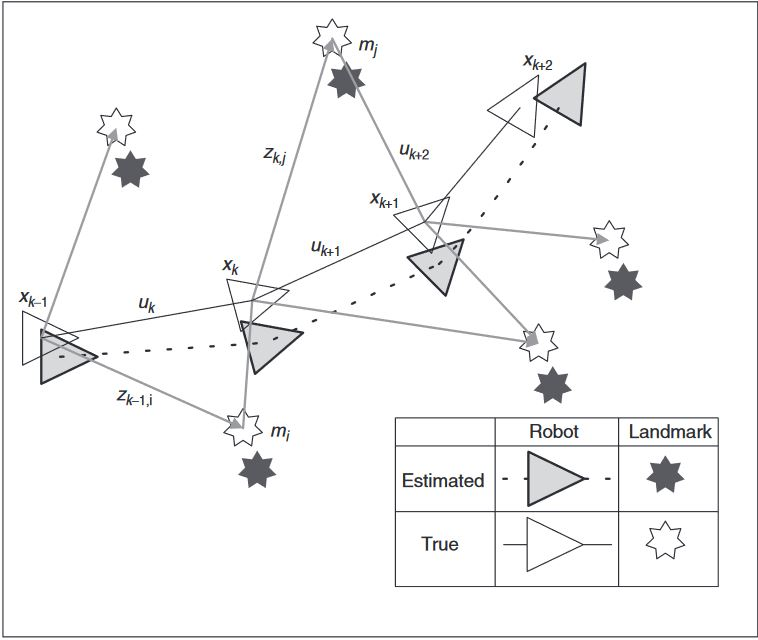
\includegraphics[width=0.5\textwidth]{figures/02marco_conceptual/slam_definicion.JPG}
    \caption{\label{fig:problema_slam} Problemática general del SLAM} 
    Fuente: \cite{durrant-whyte_simultaneous_2006}
\end{figure}

La aplicación de esta técnica es de suma importancia en entornos exteriores o no controlados, sin embargo, se siguen utilizando en la investigación en ambientes controlados por sus amplias capacidades. Es por ello, que la investigación de la técnica, la ha convertido en una de las más esenciales a la hora de construir un robot y estudiar el movimiento autónomo de estos.

Actualmente, se pueden identificar 3 grandes líneas de investigación (según de donde o como se obtenga la información para localizarse y producir el mapa) las que se pueden identificar como \textit{Laser SLAM}, \textit{Visual SLAM} o \textit{SLAM 3D} dependiendo de los sensores que se utilicen para obtener la información correspondiente. Si bien existen diversas ramificaciones de pseudo-algoritmos, el algoritmo básico planteado en el Algoritmo \ref{alg:Algoritmo SLAM}

\begin{algorithm}[H]
\centering
    \begin{algorithmic}[1]
        \Require $map\_size$
        \vspace{1mm}
        \hline
        \vspace{1mm}
        \State slam = init\_slam(map\_size)
        \For{n = 0; ;n+ +}
            \State image = acquire\_frame()
            \State predict(slam, robot\_model)
            \State j = 0
            \State lmk\_list = select\_lmks(slam)
            \State correl\_list = correl\_lmks(lmk\_list, frame)
            \For{i = 0, i < size(correl\_list) and j < nb\_correct; i++}
                \If{score(correl\_list[i]) > correl\_threshold}
                    \State correct\_slam(correl\_list[i])
                    \State j ++
                \EndIf
            \EndFor
            \State feature\_list = detect\_features(frame)
            \State j = 0
            \For{i = 0; i < size(feature\_list) and j < nb\_init; i++}
                \If{init\_lmk(feature\_list[i]}
                    \State j++
                \EndIf
            \EndFor
        \EndFor
        \vspace{1mm}
    \hline
    \vspace{1mm}
    \end{algorithmic}
\caption{Pseudocódigo algoritmo SLAM}
Fuente: \cite{vslam_2018}
\label{alg:Algoritmo SLAM}
\end{algorithm}

\begin{itemize}
    \item \textbf{\textit{Laser SLAM: }} También conocida como SLAM, corresponde a la técnica que utiliza láser o lidares para lograr el mapeo y la localización en un entorno. La noción de localización y mapeo de forma simultánea fue descrita inicialmente en 1986, pero no fue hasta la década del 2000 donde se logró implementar por primera vez en un automóvil autónomo.
    
    Los beneficios de utilizar láser como medio para obtener información es que son altamente confiables y el mapa creado no presentará errores acumulativos. Por otra lado, desde el punto de vista económico, existe una alta variedad de precios, por lo que la elección dependerá de los requisitos que se quieran satisfacer.
    
    \item \textbf{\textit{Visual SLAM: }} Técnica conocida como VSLAM corresponde a la utilización de cámaras (la única información que se tiene es la proveniente de las cámaras)  para generar una representación visual generando particiones visuales de lo observado y comparándolas con lo ya observado. Gracias a esta información se podrá tener más información sobre el entorno, sin embargo, la técnica está orientada a utilizarse en ambientes interiores debido a que la luz puede afectar y perjudicar el desempeño del algoritmo.
    
    El primer algoritmo en esta línea de investigación fue desarrollado el año 2003 llamado MonoSLAM, debido a que utilizaba una sola cámara monocular para obtener la información, cual tenía 6 grados de libertad \footnote{ Llámese grados de libertad a la cantidad de movimientos independiente que tiene una estructura, en un espacio tridimensional, el máximo son 6: 3 relacionados a la traslación y 3 relacionados a la rotación.}. Luego, tras los beneficios encontrados por las siguientes versiones del algoritmo, durante los años 2010 y 2016 se produjeron bastantes progresos con respecto a la técnica VSLAM \cite{4160954}.
    
    \item \textbf{\textit{SLAM 3D: }}  Por otra parte, esta nueva línea de investigación descrita por primera vez por Teng Hooi \cite{chan_lidar-based_2021}, en donde se realiza una aproximación tridimensional a la técnica SLAM agregando un ``grado de libertad" a los lidares (Esto se realizó utilizando lidares 3D \footnote{Un lidar 3D permite generar un mapeo tridimensional del entorno a través de una refracción interna del láser. }, en vez de las cámaras oculares), de esta manera el algoritmo puede generar un entorno tridimensional y navegar sobre él como se puede observar en la Figura \ref{fig:3D_SLAM} en donde en la parte superior se encuentra el entorno simulado y en la parte inferior la visualización 3D del entorno y la ruta de navegación realizada.
    
    Si bien existen diversos algoritmos relacionados con esta nueva línea de investigación, unos más complejos, otros con más variable y otros con más requerimientos, se puede encontrar un denominador común como lo es el algoritmo básico que se puede observar en el Algoritmo \ref{alg:Algoritmo 3DSLAM}.
\end{itemize}

\begin{figure}[H]
    \centering
    \begin{subfigure}[b]{0.45\textwidth}
    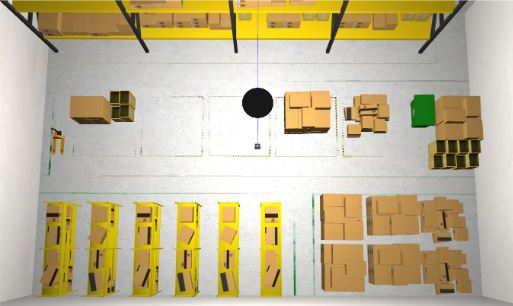
\includegraphics[width=\textwidth]{figures/02marco_conceptual/slam3d_1.JPG}
    \caption{Ambiente simulado}
    \label{fig:slam3d_1}
    \end{subfigure}
    \hspace{5mm}
    \begin{subfigure}[b]{0.45\textwidth}
    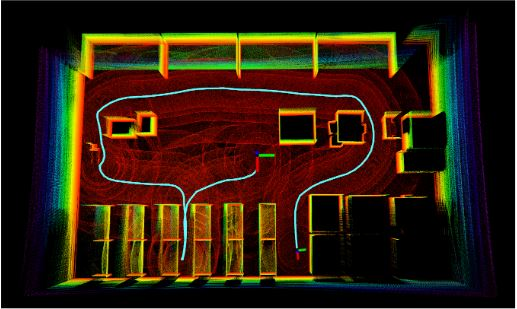
\includegraphics[width=\textwidth]{figures/02marco_conceptual/slam3d_2.JPG}
    \caption{Mapa generado por el algoritmo LIO-SAM}
    \label{fig:slam3d_2}
    \end{subfigure}
    \caption{ Reconstrucción tridimensional de un ambiente}
    Fuente: \cite{chan_lidar-based_2021}
    \label{fig:3D_SLAM}
\end{figure} 


\begin{algorithm}[H]
\centering
    \begin{algorithmic}[1]
        \Require $C$
        \Require $V_i$ points
        \Require $C_i$ plane
        \Require $S_c$
        \Require $N_i$
        \Require $\tau_\tau$
        \Require $\tau_m$
        \vspace{1mm}
        \hline
        \vspace{1mm}
        \State $C$ \leftarrow createGridCellStructure($S_c$)
        \ForAll{$v_i \in V$}
            \State writeToCorrespondingGridCell($v_{i}$, $C$)
        \EndFor
        \ForAll{$C_i \in C$}
            \State $C_i$ plane\leftarrow planarSegRansac($C_i$ points)
        \EndFor
        \While{$True$}
            \State $C_x \leftarrow getMinError(C)$
            \State $q \leftarrow merge(q, C_x)$
            \State $q \leftarrow growRegionGBS(q, C)$
            \While{ $q \neq \emptyset$}
                \State $q \leftarrow growRegionGBS(q, C)$
            \EndWhile
        \EndWhile
        \vspace{1mm}
    \hline
    \vspace{1mm}
    \end{algorithmic}
\caption{Pseudocódigo general para algoritmo 3D SLAM }
Fuente: \cite{3dslam_2018}
\label{alg:Algoritmo 3DSLAM}
\end{algorithm}

El problema de localización ha sido la piedra angular en la construcción de robots desde la década de los 50, dicho problema se puede entender como la tarea de que el robot estime la posición en un ambiente conocido a través de diversos sensores, sin embargo, un robot totalmente inteligente debe ser capaz de explorar los ambientes desconocidos donde la posibilidad de obtener tener un mapa del entorno está limitada o es inaccesible \cite{taheri_slam_2021}. En ambientes exteriores, uno de los elementos que se utiliza para la estimación de la posición es el \textit{Global Positioning System} o GPS, sin embargo, dicho sensor no es utilizable en un robot que se utilice en ambientes \textit{indoor}, por lo que se requerían nuevos sistemas y algoritmos para proveer y generar un mapa del entorno a la vez que se realiza una estimación de la posición, es bajo esta problemática que los algoritmos SLAM son creados, es decir, los algoritmos SLAM fueron creados para darle solución a los escenarios donde no se tiene referencia del mapa previamente \cite{thrun_probabilistic_2005}.

Durante los últimos 25 años, investigaciones y experimentos con algoritmos SLAM han llevado a la técnica a ser una de las más estudiadas y utilizadas en los robots modernos tanto para ambientes de interior como también para ambientes de exterior, llevando incluso los límites más allá de las fronteras iniciales y aplicándolos a ambientes aéreos, acuáticos, subterráneos, entre otros debido a los múltiples beneficios encontrados. En este tiempo, los algoritmos SLAM diseñados utilizan una seria de sensores como lo son las cámaras \textit{Red, Green and Blue} o RGB, sensores ultrasónicos, LIDARES, entre otros para estimar la posición en ambientes bidimensionales o tridimensionales \cite{li_topology_2016}. Si bien en dicho documento, se establece que el SLAM 2D es un problema que ya está resuelto, sin embargo, la creación de nuevas tecnologías, nuevos técnicas y requerimientos han reabierto el problema, debido a que la precisión, la velocidad y los nuevos datos que se generan por el avance de la tecnologías implicaban nuevas mejoras a los algoritmos creados con anterioridad \cite{taheri_slam_2021}.

En el año 2007, se aborda la problemática, sin embargo, se plantea desde otro punto de vista en el cual, esta vez se considera que el mapeo y la localización son tareas paralelas \cite{klein_parallel_2007}, no fue hasta esta investigación en donde los algoritmos SLAM fueron conocidos. Además de dar una primera noción sobre una posible solución a la localización y mapeo de manera simultánea, en dicho paper se establecen las implicancias de tener un mapa adecuado las cuales se pueden resumir en los siguientes 3 puntos:
\begin{enumerate}
    \item En primer lugar, los mapas son necesarios para poder realizar la planificación de rutas, evitar obstáculos, establecer puntos de interés, entre otros elementos. 
    \item En segundo lugar, bastantes aplicaciones de robots son justamente creadas para la construcción de mapas, por lo que se pueden encontrar robots cuyos objetivos son la construcción del mapa.
    \item Por último, que tan adecuada, eficiente, precisa y rápida es la localización del robot en el entorno depende significativamente de la precisión del mapa.
\end{enumerate}

Tal cual como se puede identificar en su nombre, los algoritmos SLAM presentan dos sub-algoritmos, algoritmos de localización y los algoritmos de mapeo \textit{(algoritmos de localización y mapeo simultáneos)}, los cuales inicialmente (década de los 50) se consideraban como elementos separados, sin embargo, las aproximaciones modernas, sobretodo aquellas que se han realizado en la última década, han mostrado que estos dos sub-algoritmos dependen directamente uno del otro, por lo que se podrían considerar como una sola problemática, por una parte para realizar un mapeo correcto, se requiere una correcta localización, mientras que para localizarse correctamente, se requiere un mapa preciso, es por ello, que los algoritmos SLAM abordan la problemática de localización y mapeo de manera simultánea. 

Las técnicas utilizadas para estimar la posición y así resolver el problema de localización se pueden clasificar en 2 tipos según el enfoque que se tenga: enfoque probabilístico y enfoque no probabilístico, mientras que los primeros al utilizar la información de los sensores estiman en base a una probabilidad de donde está el robot, los segundos utilizan un enfoque de filtrado de partículas y filtrados de Kalman. Estos últimos, específicamente aquellos que utilizan el filtro de Kalman, poseen una gran ventaja a la hora de estimar la posición debido a que son simples de implementar, lo que conlleva a que sean los algoritmos predilectos a la hora de utilizarlos, sin embargo, existen dos grandes problemas: Por una parte, los algoritmos que implementan dicho filtro son susceptibles a los errores acumulativos en la estimación de la posición, por otra parte, estos algoritmos solo se pueden utilizar en sistemas lineales \footnote{La gran mayoría de los sistemas robóticos son no lineales, sin embargo, estos se pueden linealizar rápidamente utilizando herramientas creadas para utilizar el filtrado de Kalman como lo es el \textit{Extended Kalman Filter} o EFK.}. 

\begin{figure}[h]
    \centering
    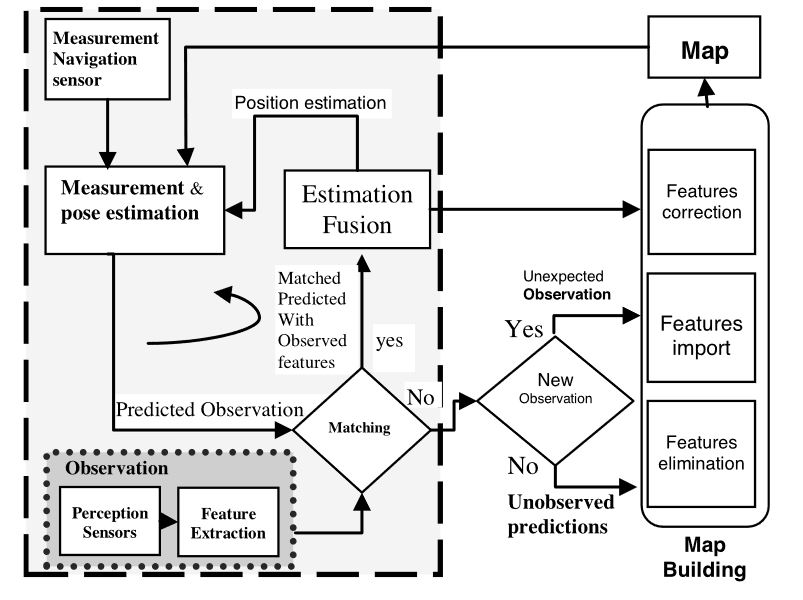
\includegraphics[width=0.8\textwidth]{figures/02marco_conceptual/esquema_general_slam.JPG}
    \caption{\label{fig:esquema_slam} Esquema general de los algoritmos SLAM} 
    Fuente: \cite{john_sonar_1992}
\end{figure}

Con el paso del tiempo y la optimización de las técnicas utilizando el filtrado EFK se obtuvieron mejores resultados, sin embargo, el modelo inicial se mantuvo intacto, el cual se puede observar en la figura \ref{fig:esquema_slam}. En términos prácticos se puede resumir en los siguientes 5 pasos: 
\begin{enumerate}
    \item A partir de los primeros datos recibidos por parte de los sensores, se construye una primera versión del mapa.
    \item Se estima una primera posición en este mapa inicial.
    \item A partir del movimiento del robot, tanto la localización como el mapa se van actualizando mediante marcadores.
    \item Se asocian los nuevos puntos de interés y se realiza una relación entre los marcadores antiguos y los nuevos para actualizar el mapa.
    \item Por cada iteración, se actualiza la ruta planificada por el algoritmo utilizando el mapa que se va generando y la información de los sensores, hasta que el robot llega a su objetivo.
\end{enumerate}

La arquitectura detrás del algoritmo SLAM se puede separa en 4 elementos esenciales, los cuales se encargan desde la obtención de los datos hasta la producción del mapa y la estimación de la posición. Estos 4 elementos, se pueden observar en la Figura \ref{fig:arquitectura_slam}. En detalle, cada elemento tiene sus tareas respectivas y sigue un flujo definido:
\begin{enumerate}
    \item \textbf{\textbf{Sensory input: }} Corresponde a todos los datos provenientes de los sensores, como lo son las imágenes, los datos del lidar, encoders, entre otros.
    \item \textbf{\textit{Front-End: }} En esta sección, el algoritmo toma los datos provenientes de la etapa anterior (los cuales están sin procesar), realiza la transformaciones respectivas como lo son la extracción de las características principales, asociación de datos, asociar datos entre otras funcionalidades y envía los datos a la siguiente sección.
    \item \textbf{\textbf{Back-End: }} En el Back-End, el algoritmo toma los datos enviados por el Front-End, realiza una optimización del modelo a través de un ajuste de parámetros y luego también define la posición y construye el mapa con dichos datos. A partir de estos valores, se ajustan los marcadores identificados y se le entrega un feedback al Front-End.
    \item \textbf{\textit{SLAM: }} En la última etapa, el algoritmo construye el mapa y realiza la estimación de la posición a partir de lo entregado por el Back-End.
\end{enumerate}

\begin{figure}[h]
    \centering
    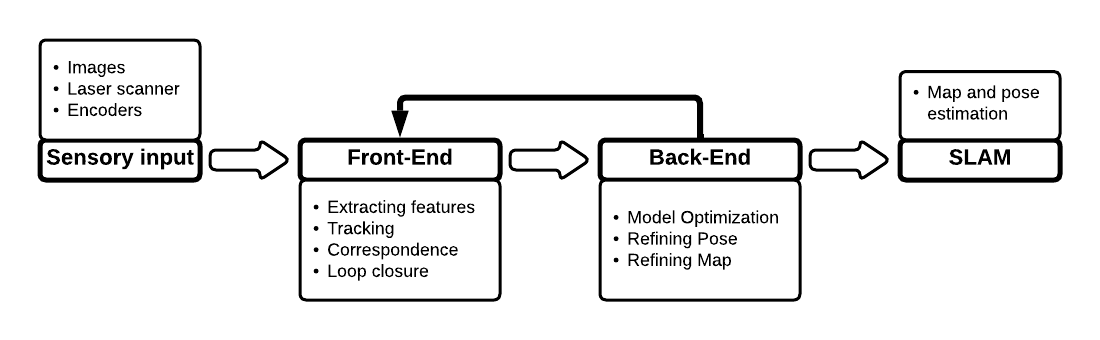
\includegraphics[width=0.8\textwidth]{figures/02marco_conceptual/arquitectura_slam.png}
    \caption{\label{fig:arquitectura_slam} Arquitectura algoritmo SLAM} 
    Fuente: \cite{taheri_slam_2021}
\end{figure}

\subsubsection{DIFICULTADES Y DESAFÍOS AL UTILIZAR SLAM}

Si bien existen una variedad de algoritmos SLAM, los autores concuerdas que por una parte el problema del SLAM es un problema en general, que aún no está resuelto y que existen 4 problemáticas en general: La asociación de los datos, La incertidumbre, el ruido o el error acumulativo y la complejidad temporal \cite{7482163}. Estas 4 problemáticas se definen a continuación: 

\begin{itemize}
    \item \textbf{La asociación de los datos: } Uno de los problemas claves a resolver en los algoritmos SLAM es la asociación de los datos, es decir, estimar correctamente los puntos y marcadores obtenidos por los sensores y asociarlos a nuevos datos. La asociación de datos permite al robot asociar el punto de origen, objetivo y la posición actual a coordenadas y referencias en el mapa \cite{problem_dissanayake_2011}.
    
    \item \textbf{La incertidumbre: } El problema de la incertidumbre hace alusión a la incerteza de los algoritmos (dado que se trabaja con algoritmos probabilísticos). En la literatura se pueden encontrar diversas definiciones de la problemática, sin embargo, se utilizará la definida en \cite{5136492}, en dónde se hace alusión a la capacidad del algoritmo de identificar las diversas rutas hacia un objetivo dependiendo de la posición en la que se encuentre. Este problema escala rápidamente en los ambientes reales en donde existen múltiples rutas para navegar desde un punto inicial hasta un punto final y existen obstáculos de diverso origen.
    
    \item \textbf{El ruido o el error acumulativo: } Los sensores cumplen un papel fundamental en los algoritmos SLAM debido a que la información para crear el mapa y localizarse proviene directamente de ellos. En la literatura se realiza un extenso estudio sobre la problemática \cite{bordoni_noise_1990} en donde se define como el ruido que tienen los sensores y por ende, el error asociado a la obtención de datos lo que termina provocando errores en el cálculo a la hora de estimar la ubicación y calcular los puntos de referencias.
    
    \item \textbf{La complejidad temporal: } Para evaluar el rendimiento de un algoritmo, se utiliza lo que comúnmente se conoce como complejidad temporal. En los algoritmos SLAM dicha complejidad se calcula aproximadamente en función de la cantidad de puntos utilizados para estimar la posición y los cálculos correspondientes para esta estimación. Dada la urgencia de tener algoritmos que funcionen en tiempo real, es un problema esencial en la literatura \cite{977154}. Actualmente existen una variedad de algoritmos que cumplen con diversos requisitos, donde se destaca el propuesto en \cite{4399179} con una complejidad computacional de $O(n)$, sin embargo, con un coste computacional bastante alto \footnote{Llámese coste computacional al coste asociado a los recursos consumidos por el algoritmo en cuestión.}.
\end{itemize}

















